\section{Théorème de Thalès}
    \subsection{Énoncé}
        \begin{theoreme}[\admis]
            Si dans un triangle $ABC$ :
            \begin{itemize}
                \item Deux droites $(d)$ et $(d')$ sont sécantes en un point $A$.
                \item $M$ est un point du côté $[AB]$ distinct de $A$ et $B$.
                \item $N$ est un point du côté $[AC]$ distinct de $A$ et $C$.
                \item les droites $(BC)$ et $(MN)$ sont parallèles.       
            \end{itemize}
            \medskip
            alors les rapports $\dfrac{AM}{AB}$ , $\dfrac{AN}{AC}$ et $\dfrac{MN}{BC}$ sont égaux.
        \end{theoreme}

        \begin{remarque}
            En fait ce théorème traduit la proportionnalité entre les longueurs des côtés des triangles $ABC$ et $AMN$.
            Les longueurs des côtés du triangle $AMN$ sont {\em proportionnelles} aux côtés correspondants du triangle $ABC$.

            \medskip
            \begin{tabular}{|p{6cm}|c|c|c|}
            \hline 
            Longueurs des côtés de ABC & AB & AC & BC \\ 
            \hline 
            Longueurs correspondantes des côtés de AMN & AM & AN & MN \\ 
            \hline 
            \end{tabular} 

            \medskip
            Les rapports $\dfrac{AB}{AM}$ , $\dfrac{AC}{AN}$ et $\dfrac{BC}{MN}$ sont donc aussi égaux.
        \end{remarque}
    
    \subsection{Configurations de Thalès}
        \emoji{light-bulb} \color{black}{\dashuline{\color{black}{Les droites en pointillés noirs sont parallèles.}}}
        \color{black}

        \hspace*{-1cm}
        % \vspace*{-4cm}
        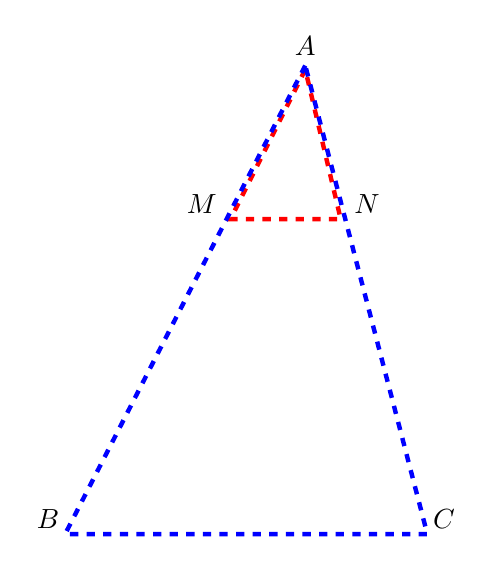
\begin{tikzpicture}[scale = 0.5]        
            % \draw[help lines, color=black!30, dashed] (0,0) grid (12,14);        
            \coordinate[label=above:$A$] (A) at (7,13);
            \coordinate (A1) at (7,12.9);
            \coordinate[label=above right:$C$] (C) at (10,1);
            \coordinate (C1) at (10.1,1.1);
            \coordinate[label=above left:$B$] (B) at (1,1);
            \coordinate (B1) at (0.9,1.1);
            \coordinate[label=above left:$M$] (M) at (5,9);
            \coordinate (M1) at (5.1,9.1);
            \coordinate[label=above right:$N$] (N) at (8,9);
            \coordinate (N1) at (7.9,9.1);

            \tkzDrawSegment(A,B);
            \tkzDrawSegment(A,C);
            \tkzDrawSegment(B,C);        
            \draw[dashed, color=red, ultra thick] (A1)--(M1)--(N1)--(A1);
            \draw[dashed, color=blue, ultra thick] (A)--(B1)--(C1)--(A);
            \tkzDrawLine[dashed, color=black, ultra thick, add = 0.8 and 0.8](M,N);
            \tkzDrawLine[dashed, color=black, ultra thick](B,C);
        \end{tikzpicture}
        \hspace*{10mm}
        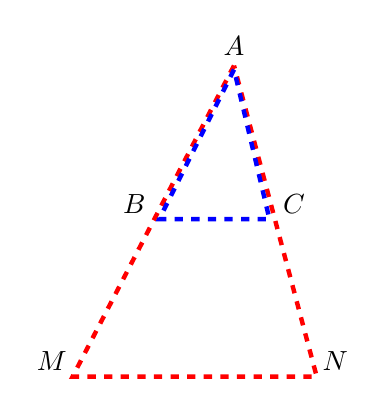
\begin{tikzpicture}[scale = 0.5]
            % \draw[help lines, color=black!30, dashed] (0,0) grid (12,14);        
            \coordinate[label=above:$A$] (A) at (7,13);
            \coordinate (A1) at (7,12.9);
            \coordinate[label=above right:$N$] (N) at (9,5);
            \coordinate (N1) at (9.1,5.1);
            \coordinate[label=above left:$M$] (M) at (3,5);
            \coordinate (M1) at (2.9,5.1);
            \coordinate[label=above left:$B$] (B) at (5,9);            
            \coordinate (B1) at (5.1,9.1);
            \coordinate[label=above right:$C$] (C) at (8,9);
            \coordinate (C1) at (7.9,9.1);
            

            \tkzDrawSegment(A,M);
            \tkzDrawSegment(A,N);
            \tkzDrawSegment(M,N);
            \tkzDrawSegment(B,C);
            \draw[dashed, color=red, ultra thick] (A)--(M1)--(N1)--(A);
            \draw[dashed, color=blue, ultra thick] (A1)--(B1)--(C1)--(A1);
            \tkzDrawLine[dashed, color=black, ultra thick](M,N);
            \tkzDrawLine[dashed, color=black, ultra thick, add = 0.5 and 0.5](B,C);
        \end{tikzpicture}

    \subsection{Exemple de rédaction}

        \begin{methode*1}[Calculer une longueur]
            \begin{multicols}2
                \begin{itemize}
                    \item Identifier les deux triangles.                    
                    \item Vérifier les appartenances.                     
                    \item Déterminer les droites parallèles,
                    
                    éventuellement le justifier.                    
                    \item Écrire l'égalité des trois rapports.
                    \item Déterminer les longueurs inconnues.
                \end{itemize}
            \end{multicols}

            \exercice

            \begin{minipage}{8cm}
                \begin{tikzpicture}[scale=1]
                    % \draw[help lines, color=black!30, dashed] (0,0) grid (8,12);        
                    \coordinate[label=above:$O$] (O) at (4,6);
                    \coordinate (O1) at (4,5.9);
                    \coordinate (O2) at (4,6.1);
                    \coordinate[label=left:$N$] (N) at (2,1);
                    \coordinate (N1) at (1.9,0.95);
                    \coordinate[label=right:$S$] (S) at (10,1);
                    \coordinate (S1) at (10.15,0.95);
                    \tkzDefPointBy[homothety=center O ratio 0.6](N) \tkzGetPoint{M};
                    \tkzDefShiftPoint[M](0.1,0.1){M1}                    
                    \tkzDefPointBy[homothety=center O ratio 0.6](S) \tkzGetPoint{V};
                    \tkzDefShiftPoint[V](-0.2,0.1){V1}  
                    \tkzLabelPoints[left](M);
                    \tkzLabelPoints[right](V);
                    \draw(O)--(N)--(S)--(O)--(V)--(M);
                    \draw[dashed, ultra thick, color=red] (O1)--(M1)--(V1)--(O1);
                    \draw[dashed, ultra thick, color=blue] (O2)--(N1)--(S1)--(O2);
                    \begin{scope}[ dim style/.append style={red, dashed},
                        dim fence style/.style={red, dashed}]                
                        \tkzDrawSegment[dim={\(\Lg{13}\),-10mm,sloped,above=1mm}](S,O);
                        \tkzDrawSegment[dim={\(\Lg{9}\),-5mm,sloped,above=1mm}](V,O);
                        \tkzDrawSegment[dim={\(\Lg{7}\),-5mm,below=1mm}](M,V);
                    \end{scope}
                \end{tikzpicture}
            \end{minipage}
            \begin{minipage}{8cm}
                \begin{itemize}
                    \item Les droites $(MV)$ et $(NS)$ sont parallèles.
                    \item $M \in [ON]$ et $V \in [OS]$.
                \end{itemize}
                Calculer la longueur $NS$.
            \end{minipage}
            
            \correction
            Dans la configuration ci-dessus : 
            \begin{itemize}
                \item les deux triangles de la configurations sont \textcolor{red}{$OMV$} et \textcolor{blue}{$ONS$}.
                \item $M \in [ON]$ et $V \in [OS]$.
                \item les droites $(MV)$ et $(NS)$ sont parallèles.
                
            \end{itemize}
            D'après le théorème de Thalès, on peut donc écrire l'égalité des trois rapports :
            $$\frac{\textcolor{red}{OM}}{\textcolor{blue}{ON}}=\frac{\textcolor{red}{OV}}{\textcolor{blue}{OS}}=\frac{\textcolor{red}{MV}}{\textcolor{blue}{NS}}\qquad\mbox{c'est à dire}\qquad\frac{\textcolor{red}{OM}}{\textcolor{blue}{ON}}=\frac{\textcolor{red}{9}}{\textcolor{blue}{13}}=\frac{\textcolor{red}{7}}{\textcolor{blue}{NS}}$$

            % \begin{minipage}{8cm}
                $$\mbox{\bf Pour le calcul de NS}$$
                $$\mbox{on utilise} \quad \dfrac{9}{13}=\dfrac{7}{NS}$$
                \begin{center}
                    {\bf Les produits en croix sont égaux}
                \end{center}
                $$\Eqalign{9\times NS&=13\times7}$$
                \begin{center}
                    {\bf On divise les deux membres par $9$}
                \end{center}
                $$\Eqalign{NS&=\frac{13\times7}{9}\simeq\Lg{10.1}\cr}$$
            % \end{minipage}
        \end{methode*1}